\chapter{黄 疸}

黄疸是指血清中胆红素浓度升高,致使巩膜、皮肤和黏膜发黄的症状和体征。正常血清胆红素浓度最高为17.1μmol/L(1.0mg/dl),其中结合胆红素3.42μmol/L、非结合胆红素13.68μmol/L。胆红素在17.1~34.2μmol/L(1.0~2.0mg/dl)时,临床不易被觉察,称隐性黄疸,超过34.2μmol/L时出现黄疸。黄疸须与球结膜下脂肪积聚及胡萝卜素血症相区别。

\section{【黄疸的分类、诊断步骤和诊断思路】}

按引起黄疸的病因,可归纳为4大类,即:溶血性黄疸、肝细胞性黄疸、胆汁淤积性黄疸和先天性非溶血性黄疸。按胆红素性质分类,可分为以非结合胆红素增高为主的黄疸和以结合胆红素增高为主的黄疸2大类。临床上对黄疸病因的鉴别诊断一般是在详细病史询问和体格检查基础上,以胆红素增高类型的区分为起点,结合基本的实验室筛查(主要反映肝细胞损害及功能的指标和反映胆汁淤积的指标),可大致估计黄疸的病因属哪一类(表\ref{tab27-1})\footnote{TB:总胆红素;CB:结合胆红素;PT:凝血酶原时间}。在大致区分黄疸病因分类的基础上,再根据需要选择一些病因特异的实验室和辅助检查进行诊断和鉴别诊断,则黄疸的具体病因多可查明。

\begin{table}[htbp]
\centering
\caption{三大类黄疸实验室检查的区别}
\label{tab27-1}
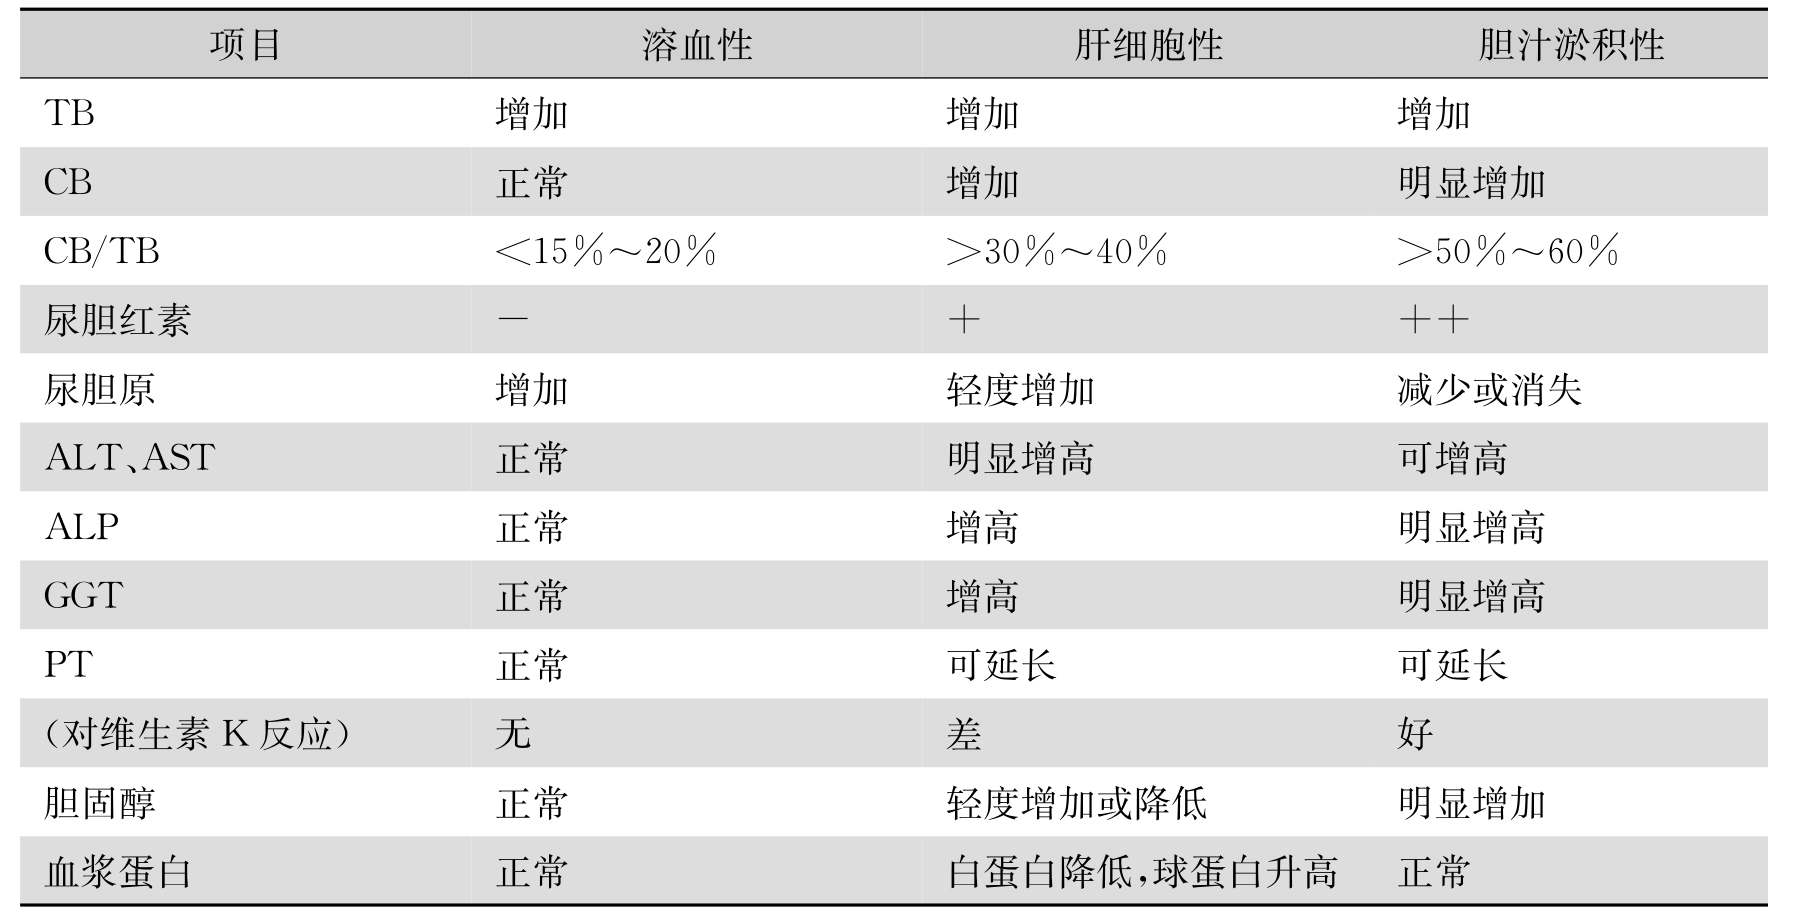
\includegraphics[width=5.96875in,height=3.05208in]{./images/Image00150.jpg}
\end{table}


值得指出的是,从表\ref{tab27-1}可以看出,肝细胞性黄疸与胆汁淤积性黄疸的区分主要是胆红素升高的类型和血清酶学改变的不同,但两者常有重叠,鉴别有时会有一定困难。因此,需要密切结合临床表现,并在此基础上选择适当的相关检查进行鉴别。B超检查简便易行,对肝外胆汁淤积的诊断有特别价值,故常作为两者鉴别的常规筛查项目。先天性非溶血性黄疸临床少见,特点是大多全身状况良好,胆红素升高多不伴血清酶学改变,其诊断和鉴别诊断要点详见下文。

\section{【黄疸的伴随病征】}

\subsection{1.发热}

见于急性胆管炎、肝脓肿、钩端螺旋体病、败血症及其他严重感染性疾病。病毒性肝炎可先有发热后出现黄疸。急性溶血时先出现高热、寒战后有黄疸。

\subsection{2.腹痛}

胆石症或胆道蛔虫发作时右上腹阵发性绞痛。持续右上腹钝痛或胀痛多见于肝脓肿、肝癌。上中腹及腰背痛见于胰腺炎或胰腺癌。

\subsection{3.肝大}

在肝病多见。急性肝炎呈轻至中度肿大,质软而有触痛。慢性肝炎肝大可呈硬度增加、边缘变钝。肝硬化时肝大不明显,触及部位质硬,表面有结节感。肝癌时肝大常明显、质坚硬、表面凹凸不平。

\subsection{4.脾大}

病毒性肝炎、钩端螺旋体病、败血症、肝硬化及溶血性贫血均可有不同程度脾大。

\subsection{5.胆囊肿大}

癌性阻塞性黄疸(如胰头癌、壶腹周围癌、胆总管癌)时胆囊肿大且呈表面平滑、可移动性和无压痛特点。急性胆囊炎时胆囊肿大有触痛伴阳性Murphy征。

\subsection{6.腹水}

见于肝硬化、肝癌、重型肝炎等。

\section{【辅助检查】}

\subsection{1.B超检查}

对发现肝、胆、胰、脾等病变有帮助,对肝外胆管阻塞引起的胆管扩张征象在黄疸鉴别诊断中有特别价值。简便易行,常作为首选的筛查手段。

\subsection{2.CT上腹部扫描}

可显示肝、胆、胰、脾等病变。分辨率高,对B超不能确诊或B超检查阴性的病变诊断意义更大。

\subsection{3.内镜下逆行胰胆管造影(ERCP)和经皮肝穿刺胆管造影(PTC)}

能清晰显示胆管(ERCP并能显示胰管),可确定胆道梗阻的存在、部位及性质,因此对胆汁淤积性黄疸的诊断和鉴别诊断有重要价值。PTC创伤较大,适用于不宜行ERCP而有胆管扩张者。

\subsection{4.磁共振胰胆管成像(MRCP)}

诊断价值与ERCP相仿且为无创性。

\subsection{5.超声内镜}

可提高超声对胆、胰病变的分辨率。

\subsection{6.肝穿刺活检}

有助疑难黄疸病例如肝脏性质不明病灶、不明原因肝大、肝内非梗阻性与梗阻性胆汁淤积、Dubin-Johnson综合征等的诊断和鉴别诊断。常见并发症为出血和胆汁外溢,故对凝血机制障碍及严重胆汁淤积者要慎重并做好术前准备。某些病例可在腹腔镜直视下行肝活检。

\subsection{7.剖腹探查}

对上述各种检查仍无法诊断,黄疸进行性加深,而又高度怀疑肝外胆管阻塞者可考虑进行。

本章所述及的黄疸类型主要是肝细胞性黄疸及与内科关系较大的胆汁淤积性黄疸,并按表\ref{tab27-2}次序叙述。

\begin{table}[htbp]
\centering
\caption{黄疸疾病的分类}
\label{tab27-2}
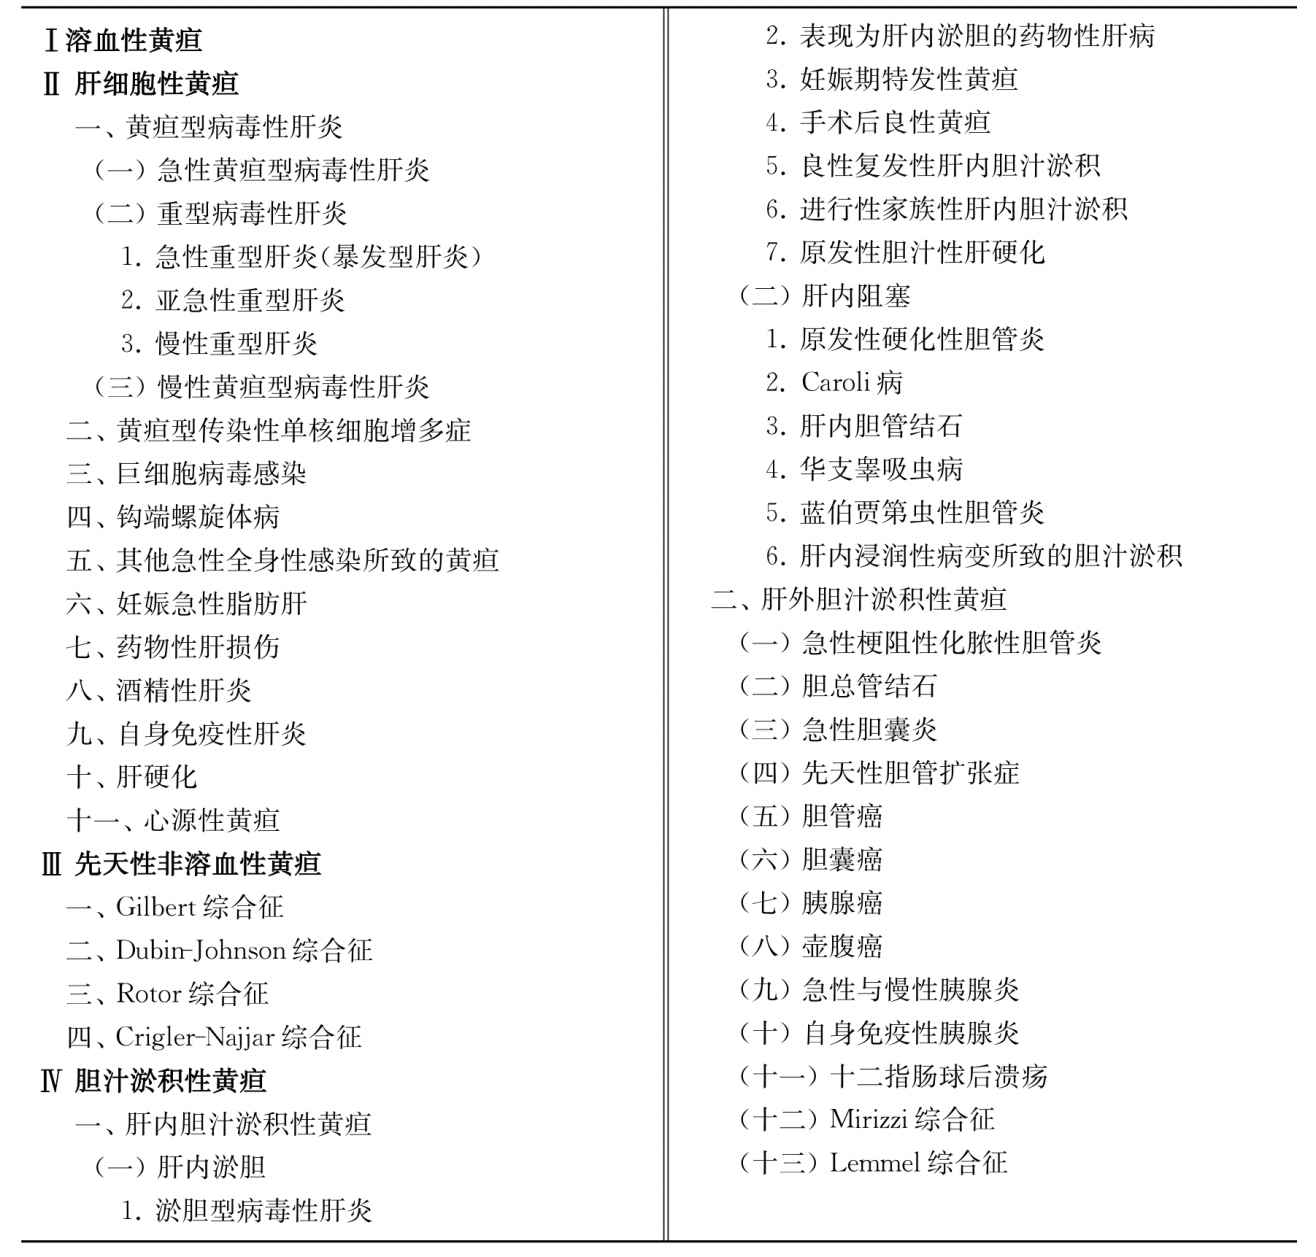
\includegraphics[width=6in,height=5.73958in]{./images/Image00151.jpg}
\end{table}

\protect\hypertarget{text00213.html}{}{}

\section{88 溶血性黄疸}

溶血性黄疸的皮肤与黏膜黄染通常为轻度,呈浅柠檬黄色,且常因贫血而伴有皮肤苍白。溶血性黄疸的原因是:红细胞本身的内在缺陷,或红细胞受外在因素所损害。受损害的红细胞可在单核-吞噬细胞系统提早破坏,或直接在血管内破坏。

溶血性黄疸的诊断(参见第113节)主要依靠下列的实验室检查所见:①血清胆红素增加,非结合胆红素增高,CB/TB<15\%~20\%。在无并发症的溶血时,血清胆红素浓度一般很少超过正常上限5倍(5mg/dl)。②尿内尿胆原含量增加。③血中网织红细胞增多。④血清铁含量增加。⑤骨髓红系统增生旺盛。

旁路高胆红素血症:又称特发性红细胞异常增生性黄疸。临床上罕见,国内仅有个案报道。血中非结合胆红素增高不是由于血循环中红细胞破坏过多引起,而是由于骨髓中红细胞前身的早标记血红蛋白分解代谢异常(无效造血)。此外可来源于非红细胞成分,主要来自肝脏,由亚铁血红素及其产物(细胞色素、肌红蛋白、含有亚铁血红素的酶)转化而来。化验检查特点是:血清非结合胆红素增高,血清铁增高,血中网织红细胞增高,肝功能正常,各项溶血检查均无异常,骨髓检查示幼红细胞增生,肝活检见肝小叶边缘区的肝细胞及Kupffer细胞内含有很多含铁血黄素颗粒。本病须与先天性非溶血性黄疸的疾病鉴别,并排除恶性贫血、地中海贫血、血卟啉病等继发性旁路性高胆红素血症。

\protect\hypertarget{text00214.html}{}{}

\section{89 肝细胞性黄疸}

\subsection{一、病毒性肝炎}

病毒性肝炎是多种肝炎病毒引起的以肝脏炎症和坏死病变为主的一组传染病。目前已明确的病原有5种,即甲型、乙型、丙型、丁型和戊型,有关己型、庚型肝炎病毒及输血传播病毒的研究仍在进行中。公认的5型肝炎病毒中,甲型肝炎病毒和戊型肝炎病毒主要引起急性肝炎或隐性感染;乙、丙、丁型肝炎病毒可引起急性肝炎、慢性肝炎或隐性感染。

按我国2000年制定的“病毒性肝炎防治方案”,病毒性肝炎的临床分型为:

1.急性肝炎 ①急性无黄疸型;②急性黄疸型。

2.慢性肝炎 ①轻度;②中度;③重度。

3.重型肝炎 ①急性重型肝炎;②亚急性重型肝炎;③慢性重型肝炎。

4.淤胆型肝炎。

5.肝炎肝硬化。

本节只讨论与肝细胞性黄疸鉴别诊断有关的急性黄疸型肝炎、慢性肝炎和重型肝炎,淤胆型肝炎及肝炎肝硬化则放在本章其他相关部分讨论。

病毒性肝炎的诊断主要根据症状(如乏力、食欲减退、恶心等)与体征(如肝大并有压痛、肝区叩击痛、黄疸)、肝功能检查异常(最常见的是ALT升高)、流行病学史及病原学检测阳性而作出,必要时可行肝活检。关于病原学检测及流行病学史参见第106节。

\subsubsection{(一)急性黄疸型病毒性肝炎}

急性黄疸型病毒性肝炎的黄疸前期为数天至一周。最突出的症状是平时很健壮的人,很快发生疲乏、食欲不振、厌油、头晕、恶心、肝区痛或不适感,伴有或不伴有发热。有些病例的主要表现为消化不良与腹泻,常被误诊为胃肠消化不良;有些主要表现为上呼吸道炎症状,常被误诊为急性上呼吸道感染;少数病例可因发热与多发性关节痛,被误诊为风湿热。黄疸前期的临床诊断比较困难,但此时血清ALT常有明显升高(阳性率达100\%),最有早期诊断价值。

黄疸出现后,患者自觉症状可反而减轻,此时除消化道症状外,主要体征为黄疸、肝大伴有触痛,肝区叩击痛也常见。也可没有明显的肝大,国内报告一组466例患者中,能触及肿大的肝脏者只占67.8\%。此期血清胆红素升高、结合与非结合胆红素均升高,尿中尿胆原排量增多与胆红素阳性。黄疸出现后,转氨酶往往开始下降。血象改变通常为白细胞计数正常或偏低,淋巴细胞相对增多,这些改变与钩端螺旋体病鉴别有重要帮助。有时血内出现相当数量的异型淋巴细胞,须与黄疸型传染性单核细胞增多症相区别,详见下文。黄疸经过一般为2~6周,有时较长。

\paragraph{附:急性病毒性肝炎的临床诊断标准(引自中华医学会传染病与寄生虫病学分会、肝病学分会2000年制定的“病毒性肝炎防治方案”)}

\subparagraph{1.急性无黄疸型肝炎}

应根据流行病学史、临床症状、体征、化验及病原学检测结果综合判断,并排除其他疾病。

(1)流行病学史:如密切接触史和注射史等。密切接触史是指与确诊病毒性肝炎患者(特别是急性期)同吃、同住、同生活或经常接触肝炎病毒污染物(如血液、粪便),或有性接触而未采取防护措施者。注射史是指在半年内曾接受输血、血液制品及用未经严格消毒的器具注射药物、免疫接种和针刺治疗等。

(2)症状:指近期内出现的、持续几天以上但无其他原因可解释的症状,如乏力、食欲减退、恶心等。

(3)体征:指肝大并有压痛、肝区叩击痛,部分患者可有轻度脾大。

(4)化验:主要指血清ALT升高。

(5)病原学检测阳性。

凡化验阳性,且流行病学史、症状和体征三项中有两项阳性或化验及体征(或化验及症状)均明显阳性,并排除其他疾病者可诊断为急性无黄疸型肝炎。

凡单项血清ALT升高,或仅有症状、体征,或有流行病学史及2)、3)、4)三项中有一项阳性者,均为疑似病例。对疑似病例应进行动态观察或结合其他检查(包括肝组织病理学检查)作出诊断。疑似病例如病原学诊断阳性,且除外其他疾病者可确诊。

\subparagraph{2.急性黄疸型肝炎}

凡符合急性肝炎诊断条件,血清胆红素>17.1μmol/L,或尿胆红素阳性,并排除其他原因引起的黄疸,可诊断为急性黄疸型肝炎。

\subsubsection{(二)重型病毒性肝炎}

\paragraph{1.急性重型肝炎}

又称暴发型肝炎。以急性黄疸型肝炎起病,2周内出现极度乏力,消化道症状明显,迅速出现Ⅱ度以上(按Ⅳ度划分)肝性脑病,凝血酶原活动低于40\%(并排除其他原因引起)可诊断之。此时黄疸急剧加深(但应注意少数病例黄疸可很浅但上述表现明显),肝浊音界进行性缩小。

在我国急性肝衰竭主要由肝炎病毒(主要是乙型)感染所致,但其他少见原因还有妊娠急性脂肪肝及中毒性肝病(如药物、毒物、酒精)等,病史及其相应的临床、化验特征可资鉴别,详见下文。

钩端螺旋体病亦可出现深度黄疸、出血及精神症状,可误诊为急性重型肝炎,应注意流行病学史并作相应的病原学检查以免误诊,鉴别要点详见下文。

\paragraph{2.亚急性重型肝炎}

以急性黄疸型肝炎起病,15天至24周内出现极度乏力,消化道症状明显,同时凝血酶原时间明显延长(凝血酶原活动度低于40\%并排除其他原因引起),黄疸迅速加深(血清胆红素每天上升>17.1μmol/L或血清胆红素>正常上限10倍)。首先出现腹水者,称腹水型;首先出现Ⅱ度以上肝性脑病者(包括脑水肿、脑疝),称脑病型。亚急性重型肝炎一般以先发生腹水为多,肝性脑病出现较晚,凝血障碍严重。晚期有难治性并发症如肝肾综合征、消化道大出血、严重感染等。

肝炎病毒感染属最常见病因,但其他少见原因亦可引起(见急性重型肝炎所述)。

\paragraph{3.慢性重型肝炎}

在慢性肝炎或肝炎肝硬化基础上发生,临床表现同亚急性重型肝炎,随病情发展而逐渐加重,达到重型肝炎诊断标准(凝血酶原活动度<40\%而血清胆红素大于正常上限10倍)。应除外甲型、戊型或其他型肝炎病毒重叠感染引起的急性或亚急性重型肝炎。

\subsubsection{(三)慢性病毒性肝炎}

急性肝炎病程超过6个月,或原有乙、丙、丁型肝炎或HbsAg携带史,本次又因同一病原再次出现临床表现及肝功能检查异常者可诊断为慢性病毒性肝炎;发病日期不明确或无肝炎病史,但肝活检组织病理学符合慢性肝炎者也可作出诊断。

根据临床表现和实验室检查将慢性肝炎分为轻、中、重3度,有助估计预后及指导治疗。

\paragraph{1.轻度}

临床症状和体征轻微或缺如。一般无黄疸,ALT在不太高的幅度内波动。休息治疗后病情好转,ALT恢复正常,但可复发。

\paragraph{2.中度}

肝病症状明显,如乏力、食欲减退、腹胀、便溏等。肝大而质韧,脾亦常肿大。可有肝病面容、黄疸、蜘蛛痣、肝掌等。ALT和AST反复或持续升高,一般在50~300U/L范围内。

\paragraph{3.重度}

上述肝病症状和体征明显而持续,但尚无门脉高压症,血清ALT和AST反复或持续升高,且伴有下述至少1项异常:白蛋白<32g/L,胆红素大于5倍正常上限,凝血酶原活动度60\%~40\%,胆碱酯酶<2500U/L。

轻度慢性肝炎相当于以往所称慢性迁延性肝炎,中度慢性肝炎相当于以往所称慢性活动性肝炎。重度慢性肝炎时肝脏多已有不同程度的纤维化,有些甚至已达早期肝硬化。临床分度与病理学改变有良好的相关性,但临床分度轻而病理学改变已相当严重的患者并不少见,因此,有条件应尽可能将临床与肝活检病理两者结合起来。

慢性病毒性肝炎须与其他原因引起的肝炎如药物性肝炎、酒精性肝病、非酒精性脂肪肝、自身免疫性肝炎、遗传代谢性肝病等进行鉴别。慢性病毒性肝炎出现黄疸时须与各种引起黄疸的慢性疾病相鉴别,由于我国HBsAg携带者相当普遍,临床上有时会将一些少见的溶血性疾病、先天性黄疸、肝内胆汁淤积性黄疸误诊为慢性肝炎。

\subsection{二、黄疸型传染性单核细胞增多症}

传染性单核细胞增多症伴有黄疸者约5\%~7\%。黄疸一般为轻度。黄疸型病例与急性黄疸型病毒性肝炎有颇多相似之点,如发热、肝脾大、食欲减退、肝功能试验不正常、血内出现异型淋巴细胞等,两者有时不易鉴别。传染性单核细胞增多症通常为流行性,咽炎较为明显,常有明显的淋巴结(尤其是颈淋巴结)肿大,胃肠道症状较轻,且有典型的血细胞形态学改变与嗜异性凝集反应效价升高,如详细检查,仍有可能与黄疸型病毒性肝炎相区别。

急性病毒性肝炎时血内可出现异型淋巴细胞,但绝对值每立方毫米一般在900个以下,持续仅为数天(发热期),以后迅速减少;在传染性单核细胞增多症时,异型淋巴细胞绝对值每立方毫米常在1000个以上,且其出现常持续2周以上。

\subsection{三、巨细胞病毒感染}

巨细胞病毒(CMV)可引起不同的感染综合征;在新生儿可引起先天性CMV综合征;在正常健康人可致单核细胞增多症;在免疫缺陷患者可引起严重的疾病综合征。健康人群中CMV抗体阳性率高达80\%~100\%,提示CMV隐性感染相当普遍,仅在免疫功能下降时病毒才激活致病。正常健康儿童或成人CMV病毒感染少见,呈单核细胞增多症表现,与EB病毒感染所致的传染性单核细胞增多症的区别为:咽痛和颈淋巴结肿大较少见,嗜异性凝集试验阴性,确诊有赖病毒分离。

\subsection{四、钩端螺旋体病}

国内报道一组钩端螺旋体病,约有70\%~90\%伴有黄疸。本病主要通过与疫水接触而感染,在农村多见于稻谷收割季节。患者以寒战、高热急骤起病,全身肌痛,尤以腓肠肌明显,严重时步行与站立均感困难,被迫卧床,此种症状有重要诊断意义。颜面与结膜往往充血。约80\%病例有不同程度的黏膜与皮肤出血。肝脾往往肿大并有触痛。全身或局部淋巴结也常肿大,尤以腹股沟淋巴结肿大为明显。发病约4~6天后出现黄疸,此时全身症状往往略有改善,而出血症状反而加重,重病例可有咯血、便血与血尿。血象呈中性粒细胞增多与左移。肝功能试验呈不同程度的异常。尿常规检查可证明蛋白尿、管型尿与血尿。严重病例可出现肝肾综合征、脑膜刺激征与昏迷。

此病的诊断须根据:①流行病学史;②急起发热、球结膜充血、腓肠肌痛、出血倾向、黄疸、淋巴结肿大与肝肾功能损害等临床表现;③确诊有赖病原学或血清学阳性结果。

黄疸出血型病例与黄疸型病毒性肝炎,特别是与重症病毒性肝炎的鉴别有一定困难。后者除黄疸之外,也常有肾脏损害、出血倾向与白细胞增多。流行病史是首先考虑的鉴别要点。重症肝炎不如钩端螺旋体病急骤,常有中毒性鼓肠、腹水等症状,而无球结膜充血、腓肠肌痛与脑膜刺激征,肺部也无异常X线征,早期肾脏损害不显著。特殊的病原学与血清学检查的鉴别诊断意义更大。

\subsection{五、其他急性全身性感染所致的黄疸}

有些急性全身性感染如大叶性肺炎、回归热、疟疾、斑疹伤寒、伤寒、波状热、急性粟粒型结核等,均可并发黄疸。黄疸一般为轻度,其原因是肝实质损害或溶血,或两者兼而有之。急性感染性疾病并发黄疸,常提示病情较重,且黄疸程度常与病情轻重相平行。大叶性肺炎并发黄疸者,病变大多位于右侧,尤以右下叶多见。

\subsection{六、妊娠急性脂肪肝}

妊娠急性脂肪肝(acute fatty liver of
pregnancy,AFLP)是妊娠末3个月内特有的少见严重产科急症,病因未明,早期不易识别,而晚期与重型病毒性肝炎鉴别常有困难。发病多为初产孕妇,常发生于妊娠30~38周内(个别可早至21周或迟至产后即刻发病)。典型临床表现为:恶心、呕吐、倦怠乏力、腹泻、烦渴多尿常为首发症状,尤以恶心、呕吐、乏力为最常见;持续约1周左右后出现黄疸并迅速加深,很快进展为暴发性肝衰竭,其中以凝血障碍性出血表现尤为明显,肾衰竭常早期出现。该病如不能早期识别并及早终止妊娠,死亡率极高,多死于消化道及(或)阴道大出血、肝性脑病及脑水肿、肾衰竭等并发症。实验室检查在典型病例见血清胆红素及ALP明显升高而转氨酶轻至中度升高,以往曾认为尿胆红素始终阴性为本病特点,但近年已不再强调。肝脏B超、CT检查提示脂肪肝有助诊断,但假阴性率高,结果正常不能排除本病。早期在凝血因子水平正常或接近正常时行经皮肝穿刺活检病理证实肝细胞微泡性脂肪变性可确诊。

本病与重型病毒性肝炎的鉴别要点是:后者有流行病学史,不限于妊娠晚期发病,病毒标记物阳性,血清转氨酶升高更为明显而DIC不常见,肝组织学示肝细胞桥状坏死及肝小叶结构破坏。事实上,HbsAg阳性患者发生的妊娠急性脂肪肝与妊娠后期发生的重型病毒性肝炎在临床上有时很难鉴别。国内一组80例妊娠合并肝病的病理学报告妊娠急性脂肪肝占18.6\%,多于急性、亚急性重型病毒性肝炎(6.2\%),因此作者建议妊娠后期发生的急性肝衰竭应更多考虑妊娠急性脂肪肝,即便两者临床上一时难于鉴别亦应及早终止妊娠(因为重型病毒性肝炎妊娠不结束多难以存活)。

妊娠急性脂肪肝的诊断标准是:①妊娠晚期发生消化道症状、黄疸、肝功能损害和暴发肝衰竭;②排除现症病毒性肝炎、药物性肝病、中毒及妊娠合并其他肝病;③肝脏病理组织学检查符合妊娠急性脂肪肝改变。

\subsection{七、药物性肝损伤}

很多药物和毒物可以通过本身或其代谢物的直接或间接作用引起肝细胞变性、坏死,或干扰胆汁代谢和排泄机制而引起肝内胆汁淤积,或两种作用兼有;亦可作用于肝内外免疫机制引起免疫性肝损害。

药物性肝损伤定义为ALT或结合胆红素升高超过2倍正常上限,伴AST、ALP(碱性磷酸酶)和总胆红素升高且其中1项超过2倍正常上限。临床上将药物性肝损伤分为急性和慢性药物性肝损伤,以急性多见,指的是病程在3个月内(淤胆型可稍长)。根据ALT与ALP升高的比值及结合胆红素与非结合胆红素升高的比值,将急性药物性肝损伤分为3型:肝细胞损伤、胆汁淤积型和混合性。我国统计,以肝细胞损伤型最常见。

引起肝病的常见药物有:解热镇痛药如对乙酰氨基酚(扑热息痛)、保泰松;麻醉药如氟烷;抗惊厥药如苯妥英;抗精神病药如氯丙嗪;抗微生物药如大环内酯类抗生素(以红霉素最常见)、四环素、磺胺类药物、抗结核药(以异烟肼和利福平最常见)、抗真菌药如酮康唑、抗病毒药如某些核苷酸类似物;抗肿瘤及免疫抑制药如硫唑嘌呤、甲氨蝶呤(长期应用引起肝纤维化)、氟尿嘧啶、各种烷化剂(如常见的环磷酰胺);心血管疾病用药如甲基多巴、胺碘酮、多种抗血脂药;内分泌药物如雌激素类固醇、雄激素及同化类固醇、口服降糖药如磺脲类、抗甲状腺药如硫脲类;各种含毒性生物碱、毒性皂苷、毒性蛋白或不明成分毒性物质的中草药及中成药。据我国统计,以抗结核药和中草药最常见。

药物引起的肝损伤表现多样,可急可慢、可轻可重,可表现为肝炎或淤胆或两者兼有;一般停药后逐渐好转,但亦有表现为急性肝衰竭而死亡者,也有见隐匿起病、慢性过程而发展为肝硬化者。鉴别诊断的关键是:认真询问用药史和分析用药与反应的时序关系:用药史与发病的时间关系(急性药物性肝病多在给药后1~4周内出现),观察停药后临床表现及化验指标的经过,再用药的反应。由过敏因素引起的药物性肝损害在初发症状时可有发热、皮疹及瘙痒,周围血嗜酸性粒细胞比例>6\%。原有基础肝病的患者不明原因肝病发作或加重,不要忽略药物或毒物诱发的可能。确立药物性肝损伤必须建立在排除其他病因引起的肝损伤基础上。

引起肝内淤积性黄疸的药物性肝病药物性肝病有其特点,将在本章下文讨论。

\subsection{八、酒精性肝炎}

长期嗜酒者,尤其是近期有持续大量饮酒史,出现下列情况时,须考虑本病:①新近出现食欲不振、乏力、恶心、呕吐、黄疸与腹痛;②肝大与触痛,有时脾大,伴有不明原因发热;③血清胆红素升高,血清转氨酶升高,GGT升高,外周血象白细胞增加。严重患者合并肝性脑病等肝衰竭表现,称为酒精性重型肝炎。肝活检是确诊本病的依据。

根据中华医学会肝脏病学会提出的酒精性肝病诊疗指南,如未作肝活检,对符合酒精性肝病诊断标准者(参见第107.4节),并符合下列诊断标准和附加项目中3项或以上,亦可作出酒精性肝炎的诊断。诊断标准:①饮酒量增加可作为发病或恶化的诱因;②AST为主的血清转氨酶升高;③血清胆红素升高(>34.2μmol/L)。附加项目:①腹痛;②发热;③外周血象白细胞增加;④ALT升高>1.5正常上限;⑤GGT增高>2正常上限。

本病在我国其实并非罕见,近年已有不少经病理组织学证实的病例报告。本病须与病毒性肝炎、自身免疫性肝炎、药物性肝炎及代谢性肝病相鉴别。我国慢性病毒性肝炎和HbsAg携带者相当普遍,判断此次发病是否主要由酒精性肝炎引起主要依靠长期大量饮酒史及肝活检病理所见。AST/ALT>2、GGT明显升高、戒酒后转氨酶及GGT下降情况等可供参考。

\subsection{九、自身免疫性肝炎}

自身免疫性肝炎是一种病因未明的以高球蛋白血症、有多种自身抗体和病理组织学上存在界面肝炎和汇管区浆细胞浸润为特征的肝脏炎症性疾病。西方国家发病较多,我国及东南亚国家少见,多见于年轻女性。本病临床表现酷似慢性活动性病毒性肝炎,但亦有无症状或临床表现轻者,或以关节炎等类似风湿性疾病为突出表现者,故常易误诊。我国以往对该病认识较少,近年报道的病例不断增加,应引起临床注意。

本病的诊断依据包括:①除外活动性病毒性感染、酒精或药物性肝损害、遗传代谢性肝病等;②血清转氨酶明显升高;③高球蛋白血症,血清γ球蛋白或IgG大于正常上限1.5倍;④血中存在自身抗体,包括抗核抗体(ANA)、抗平滑肌抗体(SMA)、抗肝肾微粒体Ⅰ型抗体(anti-LKM1)等;⑤肝活检见界面肝炎而无胆管损害、肉芽肿等提示其他肝病的病变。本病诊断的关键是要先排除其他病因引起的慢性肝病,而诊断的重要参考依据是自身抗体的存在。

\subsection{十、肝硬化}

各类型肝硬化失代偿期均可出现不同程度的黄疸。

\subsection{十一、心源性黄疸}

轻度黄疸可见于各种原因引起的右心衰竭,尤其伴有相对性或器质性三尖瓣关闭不全时。反复发作右心衰竭者,心源性黄疸的发生率增高。但血清总胆红素通常不超过3倍正常上限。

心源性黄疸的原因复杂。最主要的是由肝淤血、肝细胞缺氧,以致肝细胞对处理胆红素的功能不良所引起。

心源性黄疸主要须与散发性黄疸型病毒性肝炎相区别。心源性黄疸无肝炎接触史,无黄疸前期症状,黄疸程度较轻,黄疸随心力衰竭的加剧与好转而有明显的波动,肝增大与回缩的幅度较为显著,肝功能试验常提示实质性损害较轻,无明显的转氨酶活性增高。

\protect\hypertarget{text00215.html}{}{}

\section{90 先天性非溶血性黄疸}

以往称为家族性高胆红素血症,系指肝细胞对胆红素的摄取、结合及排泄有先天性缺陷所致的黄疸。此类黄疸临床上少见,但与其他类型黄疸的鉴别诊断甚为重要,因治疗与预后均有所不同。这些患者由于长期持续性或波动性黄疸的存在,常长期被误诊为慢性肝炎或慢性胆道疾病,致增加患者不必要的精神与物质的负担,甚至遭受不必要的手术。因此临床医生对此必须有明确的认识。

临床上如慢性波动性黄疸患者临床症状轻微且全身状况良好,肝功能试验除胆红素代谢障碍外无其他明显的异常,病程经过不符合病毒性肝炎的一般转归规律时,特别是有家族病史者,应注意此类少见的黄疸。

\subsection{一、Gilbert综合征}

本病是非结合胆红素增高血症的常见病因。属常染色体隐性遗传病,国内有多宗家族发病的报道。黄疸在青春期前少被发现,大多出现在青年期,男性多见。临床表现为慢性波动性黄疸,常因疲劳、紧张、饥饿、饮酒、女性月经期或附加感染出现或加深。常无自觉症状,或仅有轻度疲乏,全身状况良好。肝大少见,脾不肿大。化验除血清非结合胆红素升高外,各项肝功能试验均基本正常。胆红素浓度一般在正常上限3倍(3mg/dl)以下,少数可达5~8mg/dl。

本病临床上一般依据慢性间歇性黄疸、无明显症状、全身状况良好,肝功能检查仅有非结合胆红素增高,并能排除溶血性、肝细胞性及胆汁淤积性黄疸即可作出诊断。本病饥饿试验阳性、肝活检正常,但少有必要用于临床诊断。本病呈良性过程,预后良好。

本病发病机制主要与二磷酸葡萄糖醛酸转移酶缺乏而不能有效将非结合胆红素转化为结合胆红素有关,亦可能涉及肝细胞从血液摄取胆红素功能障碍。国外报道不少病例可伴有不明原因的轻度溶血性贫血,但我国少见报道。

\subsection{二、Dubin-Johnson综合征}

本病是另外一种相对较常见的胆红素代谢缺陷的常染色体隐性遗传病。与Gilbert综合征不同之处在于:本病发病机制主要是肝脏对胆红素的摄取和结合功能正常,但肝细胞对结合胆红素及其他有机阴离子(如磺溴酞钠、X线造影剂)的运输和向毛细胆管排泄功能障碍,使结合胆红素反流入血而导致高结合胆红素血症。

本病多发病于青少年,常有家族史。临床表现为慢性波动性黄疸,黄疸一般不深,可因其他疾病或服用某些药物而加重。不少患者主诉肝区隐痛,约半数可触及肿大的肝脏并有触痛。有由于上腹痛、深色小便、血清结合胆红素升高及胆囊不显影等情况,而误诊为胆道疾病。本病呈良性过程,预后良好。

血清胆红素升高一般在正常上限2~5倍(2~5mg/dl),以结合胆红素升高为主。血清碱性磷酸酶不升高以及其他肝功能试验多在正常范围。胆囊造影不显影。确诊有赖于肝穿刺活检,发现肝细胞内有大量棕黑色颗粒(免疫组化染色显示这些色素为黑色素及脂褐素成分),此外无其他重要病变。确诊本病的重要意义在于可排除其他严重肝胆疾病。

\subsection{三、Roter综合征}

本病罕见,国内曾有个案报道。为常染色体隐性遗传病。多发病于儿童。血清胆红素升高一般在正常上限2~5倍(2~5mg/dl),表现为血清结合胆红素升高或结合与非结合胆红素同时升高,但血清碱性磷酸酶、胆汁酸不升高以及其他肝功能试验正常。胆囊显影良好,肝活检无明显异常。本病可能涉及肝细胞摄取非结合胆红素及转运、排泄结合胆红素过程的功能障碍,具体机制未明。本病呈良性过程,预后良好。本病须与其他先天性非溶血性黄疸鉴别。

\subsection{四、Crigler-Najjar综合征}

本病罕见,国内有个案报告。见于新生儿或儿童。因肝细胞缺乏二磷酸葡萄糖醛酸转移酶,致不能形成结合胆红素,故血清非结合胆红素浓度很高。可并发核黄疸,预后很差。本综合征分两型,Ⅰ型为二磷酸葡萄糖醛酸转移酶完全缺乏;Ⅱ型为部分缺乏,故与Ⅰ型比较,非结合胆红素浓度较低,症状较轻,预后较好。两型的鉴别除观察患者临床表现外,可用苯巴比妥试验,Ⅰ型无反应,Ⅱ型可使血清非结合胆红素下降25\%以上。

\protect\hypertarget{text00216.html}{}{}

\section{91 胆汁淤积性黄疸}

胆汁淤积是指胆汁流动或生成障碍,以致正常胆汁不能到达十二指肠。胆汁淤积而引起的黄疸则称为胆汁淤积性黄疸。胆汁淤积可由各种病因引起,淤积可发生在肝细胞(胆汁分泌)、毛细胆管、小胆管、肝内胆管及肝外胆管各个水平。无论何种病因、淤积发生于哪一水平,胆汁淤积性黄疸的共同表现为:黄疸(早期呈金黄色,稍后呈黄绿色,晚期呈绿褐色,甚至近于黑色),皮肤瘙痒与心动徐缓,血清胆红素升高(结合胆红素升高为主),血清碱性磷酸酶升高,血清胆汁酸升高,血清胆固醇升高,而血清转氨酶多不升高或轻至中度升高(与胆红素升高不平行)。胆汁淤积还可继发脂肪吸收不良、维生素K缺乏和骨病等临床表现。

胆汁淤积性黄疸与肝细胞性黄疸的鉴别至为重要,但有时亦颇困难,鉴别要点见本章前文所述,还要结合具体疾病相关表现进行分析。

胆汁淤积性黄疸根据淤胆发生的水平,可分为肝内胆汁淤积和肝外胆汁淤积两大类。前者病因及发病机制相当复杂,近年的认识已有很大提高。后者主要由肝外胆管的阻塞引起,引起肝外胆管阻塞的常见病因为结石、寄生虫、肿瘤及胆管狭窄(炎症、发育缺陷、外来压迫及术后并发症等引起)等。两者处理方法不同(后者多可通过手术治疗),因此鉴别十分重要。鉴别的要点首先是确定是否存在肝外胆管阻塞。有时病史及临床表现可提示肝外胆管阻塞,如胆石症、胆道蛔虫或以往胆道手术史,剧烈的上腹痛,扪及肿大胆囊或腹部包块等。绝大多数肝外胆管阻塞都有胆管扩张(急性早期阻塞可无),常规B超检查即可发现。然后选择B超、CT、ERCT或PTC、MRCP、超声内镜等影像学手段来辨明阻塞的部位及病变的性质。如排除肝外胆管阻塞而拟诊为肝内胆汁淤积,主要是通过病因分析进行鉴别,必要时可结合肝活检或(及)治疗试验进行诊断。对鉴别有困难而高度怀疑肝外胆管阻塞但病因未明的病例,必要时可行手术探查,术中还可结合术中B超及胆道镜进行诊断。

\subsection{91.1 肝内胆汁淤积性黄疸}

\subsubsection{一、肝内淤胆}

\paragraph{(一)淤胆型病毒性肝炎}

淤胆型病毒性肝炎是一种少见的病毒性肝炎类型,国内一组2633例肝炎中占2\%。此型病毒性肝炎的主要临床表现为较长时间的胆汁淤积性黄疸。起病类似急性黄疸型病毒性肝炎,黄疸逐渐加深,患者感觉皮肤瘙痒,但即使起病已数周,患者并无与黄疸深度相称的严重症状。常有明显肝大。肝功能检查血清胆红素明显升高,以结合胆红素为主,凝血酶原活动度>60\%或应用维生素K肌注1周后可升至60\%以上,血清ALP、GGT、胆汁酸、胆固醇均明显升高。黄疸持续3周以上,一般不超过3~6个月,少数可迁延1年以上。本病预后良好,极少数病例可演变为继发性胆汁性肝硬化。在慢性肝炎基础上发生上述表现者,则称为慢性淤胆型病毒性肝炎。

本病诊断的关键是有流行病史及血清肝炎病毒标志物阳性,并能排除其他原因引起的肝内及肝外胆汁淤积性黄疸,特别要注意与药物性肝病鉴别。

\paragraph{(二)表现为肝内淤胆的药物性肝病}

很多药物可引起急性肝内淤胆,根据其临床和病理特点可区分为两大类:

\subparagraph{1.伴有炎症反应的急性肝内淤胆}

此型黄疸以氯丙嗪黄疸最为多见。发病机制被认为是机体对药物的变态反应,有下列几项临床特点:①黄疸的发生与剂量大小无关系,通常于用药1~4周内出现;②临床上常同时伴有发热、皮疹与嗜酸性粒细胞增多症;③黄疸持续数周至数月不等,但再度用药后黄疸很快再发。病理活检可见肝内淤胆,毛细胆管内胆栓形成,汇管区周围嗜酸性粒细胞浸润,肝实质改变甚少,主要为肝细胞气球样变、糖原消失、胆色素堆积等。

国外文献报道此病偶尔可呈慢性经过,并发展为继发性胆汁性肝硬化。

引起此型黄疸的药物还有新胂凡纳明、氯磺丙脲、硫氧嘧啶、甲巯咪唑、磺胺类药物、氯噻嗪、对氨基水杨酸、红霉素丙酸酯等,但发病率很低,一般为用药者的1\%以下。

\subparagraph{2.不伴有炎症反应的急性肝内淤胆}

此型黄疸可见于应用甲基睾酮及口服避孕药等药物之后,其结构都含有17α-烃基,临床上有下列特点:①服用此类药物达到一定剂量后,部分病例出现黄疸;②临床上无发热、皮疹与嗜酸性粒细胞增多等现象;③停药后黄疸于数天至数月内消退,再次用药常引起再发;④肝活检仅显示肝内淤胆,而无炎症反应。

\paragraph{(三)妊娠期特发性黄疸}

发生于妊娠期的黄疸并不少见,大概由于下列几种原因:①妊娠中毒症;②并发病毒性肝炎;③并发胆道感染;④药物性黄疸;⑤妊娠期特发性黄疸;⑥妊娠急性脂肪肝等。

妊娠期特发性黄疸并非少见,国内已有不少病例报告。此型黄疸原因未明。主要特征是:伴或不伴有黄疸的瘙痒,妊娠期出现,产后消失。本病对母婴一般预后良好。黄疸多出现于妊娠第3个月。首发症状通常为皮肤瘙痒,可在黄疸出现前几周发生。患者可有深色尿与白陶土样大便,黄疸约在出现第一周后达到高峰。患者全身情况尚佳。时有轻度肝大。黄疸符合肝内淤胆性,在产后1~2周内迅速消退。黄疸消退后胆囊造影正常。黄疸常在再度妊娠时重新出现。也有姐妹妊娠期复发性黄疸病例报告。

此型黄疸的临床病象、肝功能试验与肝活检所见,与氯丙嗪黄疸者基本相同,但患者无应用此类药物历史。有些人曾疑为一种隐匿型肝炎,由于妊娠而加剧。在此病时,黄疸出现于妊娠3个月的后期,除皮肤瘙痒外,其他自觉症状轻微,转氨酶正常或轻度增加,黄疸在产后迅速消退,母儿预后良好,均有助于与妊娠并发急性黄疸型病毒性肝炎相区别。

本病又须与妊娠急性脂肪肝鉴别,后者类似暴发型肝炎,预后严重,详细参考第85节。

\paragraph{(四)术后良性黄疸}

多发生在大手术后的第3天,在8~10天达高峰,历经2~3周而消退。患者无发热,无皮肤瘙痒,无明显肝大。血清结合胆红素升高,转氨酶正常或中度增高,ALP轻至中度升高。肝活检证明为肝内小叶中心性淤胆而无实质性炎症。此型黄疸预后良好。

术后良性黄疸的病因和病理因素可能是综合的,与输入红细胞裂解、血肿吸收、血流动力学改变、麻醉剂应用等因素有关。应注意,术后黄疸病因复杂,在确定术后良性黄疸前必须排除各种可引起严重后果的术后黄疸,如手术引起的胆道感染或阻塞、术后右膈下感染、术后并发病毒性肝炎、严重感染及败血症等病因。

\paragraph{(五)良性复发性肝内胆汁淤积}

本病罕见,国内尚未见报道。其临床特征为反复发作无法用其他原因解释的胆汁淤积,期间间隔以很长的无症状期。本病预后良好。病因未明,近年研究认为是隐性遗传障碍,基因缺陷被定位在18号染色体,约10\%~15\%患者有家族史。肝活检除见小叶中心胆汁淤积外,不伴有肝实质及小叶胆管的病变。本病诊断前须排除其他原因引起的胆汁淤积性黄疸。

\paragraph{(六)进行性家族性肝内胆汁淤积}

进行性家族性肝内胆汁淤积是婴幼儿的一种严重肝内胆汁淤积性疾病,属常染色体隐性遗传病。近年国外研究已能阐明本病4种类型的遗传缺陷,国内则未见报道。Ⅰ型进行性家族性肝内胆汁淤积又称Byler病,具有明显的家族性,变异被定位在18q21~22染色体。临床表现为进行性的肝内胆汁淤积,可发展至肝硬化,血清胆汁酸升高,但血清GGT下降,胆固醇正常。

\paragraph{(七)原发性胆汁性肝硬化}

原发性胆汁性肝硬化是一种慢性肝内胆汁淤积性疾病,病理学上表现为进行性、非化脓性、破坏性小胆管炎,最终发展为肝硬化。病因未明,一般认为与自身免疫有关。由于诊断水平提高,国内近年已有多组病例报道。慢性肝内胆汁淤积,全身情况较好,以皮肤瘙痒和黄疸为突出症状,肝脾明显肿大,患者多为中年女性,提示本病可能,血清线粒体抗体检测及肝活检有助诊断,参见第107.5节。

\subsubsection{二、肝内阻塞}

\paragraph{(一)原发性硬化性胆管炎}

本病少见,其特征性病理改变为胆管纤维化性炎症,大部分病例病变同时累及肝内和肝外胆管,但亦有部分病例仅累及肝外胆管或仅累及肝内小胆管。近年国内已有数十例报道。多发生青壮年男性,男女比例为2~3∶1。起病隐袭渐进,就诊时多数患者已有明显症状,主要表现为黄疸、瘙痒、右上腹痛等。少部分患者有寒战、发热,可能与合并感染有关。肝常肿大,脾可肿大,实验室检查为胆汁淤积性黄疸表现,转氨酶可轻中度升高。随病程进展,可最终发展为继发性胆汁性肝硬化。国外报道半数以上原发性硬化性胆管炎患者合并溃疡性结肠炎,但我国报道中极少发现这一现象。本病诊断主要依靠胆管造影,ERCP显示肝外、内胆管呈广泛分布、多灶性狭窄,典型者肝内胆管呈“剪树枝样”或“枯树枝样”改变。肝活检并非诊断所必需,但有助除外其他疾病,对病变仅累及肝内小胆管的原发性硬化性胆管炎患者则有助诊断,典型病理组织学所见为“洋葱皮”样改变的纤维性胆管炎。本病诊断必须排除其他引起胆管狭窄的病因如胆道结石、胆道手术后、先天性胆管扩张症、胆管癌等及原发性胆汁性肝硬化。原发性胆汁性肝硬化临床表现与本病很相似,但前者以中老年女性最常见,血清线粒体抗体阳性,肝活检有助鉴别。

\paragraph{(二)Caroli病}

又称先天性肝内胆管囊性扩张,是一种先天性畸形,属常染色体隐性遗传病。本病在我国并不罕见,已有多篇大案病例报告。约有1/4~1/3Caroli病例同时有先天胆总管囊性扩张,这种类型的Caroli病亦可视为先天性胆总管囊性扩张的一种类型(参见第91.2节)。反复发作黄疸、腹痛、发热的复发性胆管炎症状为主要临床表现,可合并胆道出血而表现为上消化道出血。B超检查有重要诊断价值。ERCP或PTC胆道造影可见肝内胆管节段性扩张呈连珠状,而受累胆管末段则正常大小而不扩张。ERCP或PTC检查易发生造影剂滞留而诱发胆道感染,目前主张以MRCP检查替代。本病常合并胆管结石,并有恶变为胆管癌倾向,已有不少合并胆管癌的报道。本病须与肝内胆管结石引起的结石梗阻上方胆管继发性扩张鉴别,后者在取去结石后扩张胆管会逐渐缩小至接近正常,而前者不能。

\paragraph{(三)肝内胆管结石}

肝内胆管结石在我国颇为常见,结石可广泛分布在两叶肝内胆管,亦可局限在某叶胆管。若结石不排出,患者可无症状或诉肝区闷胀或隐痛。当结石向肝外胆管排出引起结石梗阻时,临床表现同肝外胆管结石(参见第91.2节)。结石长期堵塞在肝内胆管,可引起胆管慢性炎性增厚,继发节段性囊性扩张,在此基础上可发生复发性化脓性胆管炎。肝内胆管结石继发感染易引起胆源性肝脓肿。长期梗阻(特别是双侧肝管梗阻)及反复感染可发展为胆汁性肝硬化。诊断主要依靠B超、CT及ERCP。

\paragraph{(四)华支睾吸虫病}

重症华支睾吸虫感染可出现轻度肝内阻塞性黄疸。十二指肠引流与粪便检查(集卵法)可检出华支睾虫卵。

广西壮族自治区曾报道12例以黄疸为主要症状的急性华支睾吸虫病,患者发病前1个月左右均曾有生食淡水鱼史。由于忽略病史询问及粪便检查虫卵,致入院时被误诊为急性黄疸型病毒性肝炎。患者主要临床表现为皮肤巩膜黄染、发热、腹胀、食欲不振,肝区痛合并肝大与触痛。粪检虫卵阳性可确定诊断。

\paragraph{(五)蓝伯贾第虫性胆管炎}

本病临床上易与慢性无黄疸型肝炎相混淆,罕见病例可有轻度黄疸。十二指肠引流检出原虫,患者经甲硝唑治疗后症状缓解,黄疸消失,可证实本病的诊断。

\paragraph{(六)肝脏浸润性病变所致的胆汁淤积}

原发性肝癌或肝转移癌、淋巴瘤、白血病、肝淀粉样变等疾病均可因病变浸润压迫肝内或(及)肝外胆管而引起胆汁淤积性黄疸。

\protect\hypertarget{text00217.html}{}{}

\subsection{91.2 肝外胆汁淤积性黄疸}

肝外胆汁淤积性黄疸常称肝外阻塞性黄疸,临床上也称为外科性黄疸,阻塞的原因为:

1.胆管内因素如结石、蛔虫、华支睾吸虫、血凝块的堵塞等。

2.胆管壁因素如胆管狭窄、胆管癌、壶腹癌、胆管炎、先天性胆管闭锁等。

3.胆管外因素如胰腺癌、胰腺炎、肝门区淋巴结转移癌的压迫等。

\subsubsection{一、急性梗阻性化脓性胆管炎}

急性梗阻性化脓性胆管炎常发生于胆管结石、胆道蛔虫病、华支睾吸虫感染、胆管瘢痕性狭窄或癌梗阻等基础之上,患者常以恶寒或寒战、高热、右上腹痛而起病,常有恶心、呕吐。疼痛可相当剧烈,多为阵发性绞痛。发热呈弛张热型或败血性热型,伴有不同程度的阻塞性黄疸,可并发感染中毒性休克。肝多轻至中度肿大,伴有压痛。脾亦有时可触及。白细胞计数常明显增多,多在20×10\textsuperscript{9}
/L以上,分类中性粒细胞占优势。如患有急性右上腹痛、高热、黄疸则称Charcot三联症,示急性化脓性胆道感染。如伴有中枢神经中毒症状、休克则称Reynolds五联症,示急性梗阻性化脓性胆管炎。

影像学检查以B超最为实用,能及时了解梗阻部位及病变性质,必要时可行CT检查。结合临床典型的五联症表现、实验室及影像学检查可作出诊断。对于不具备五联症表现,当体温持续在39℃以上、脉搏>120次/分、白细胞>20×10\textsuperscript{9}
/L、血小板降低时,即应考虑为急性梗阻性化脓性胆管炎。本病须注意与阿米巴性或细菌性肝脓肿鉴别。

\subsubsection{二、胆总管结石}

胆总管结石的临床特点是阵发性上腹绞痛后出现黄疸,过去有同样发作史。如合并感染则还有寒战和发热。黄疸的程度及持续时间,取决于胆管梗阻的程度、梗阻持续的时间及是否合并感染。如梗阻为部分或间歇性,黄疸较轻且呈波动性;完全梗阻,特别是合并感染,则黄疸明显,且可呈进行性加深。化验检查显示胆汁淤积性黄疸性质。X线腹部平片见不透X线结石影像。B超、CT检查可发现结石。ERCP对胆总管结石的诊断最为准确。本病须与其他急腹症鉴别,还要与胆管癌、壶腹癌、胰头癌等引起的阻塞性黄疸鉴别,这些疾病起病缓慢,腹痛无或较轻,黄疸呈进行性加深,B超、CT及ERCP均有助鉴别。

\subsubsection{三、急性胆囊炎}

急性胆囊炎绝大多数患者合并有胆囊结石,急性发作的典型过程为突发右上腹绞痛,常在饱餐、进油腻食物后或在夜间发作,疼痛常放射至右肩部。伴恶心和呕吐。常有轻度发热。约10\%~25\%患者可出现轻度黄疸,可能是胆红素通过受损胆囊黏膜进入血循环,或邻近炎症引起Oddi括约肌痉挛所致。若黄疸重且持续,提示有胆总管结石并梗阻的可能。B超检查见胆囊结石及胆囊炎征象。

\subsubsection{四、先天性胆管扩张症}

先天性胆管扩张症曾称为先天性胆总管囊肿,本病好发于东亚国家,我国并非罕见。胆管扩张可发生在肝内、肝外胆管的任何部位,根据胆管扩张的部位、范围和形态可分为5种类型,以Ⅰ型最常见(囊性扩张累及肝总管、全部或部分胆总管),Ⅳ型次之(肝内胆管及肝外胆管囊性扩张),Ⅴ型为仅有肝内胆管囊扩张,即为前文所述的Caroli病。典型表现为腹痛、腹部包块和黄疸三联症。对于有典型三联症和反复发作胆管炎者诊断不难,但三联症俱全者仅占少部分病例(据北京协和医院的一组70例病例统计仅占10\%),故对怀疑本病者仍需借助影像学检查。B超检查有重要诊断价值,ERCP或PTC胆道造影可确诊,但因易诱发感染现建议以MRCP代替。本病可合并胆结石,有恶变为胆管癌倾向。

\subsubsection{五、胆囊癌}

胆囊癌晚期浸润可发生黄疸,胆囊区疼痛往往先发生于黄疸,详见第76.2节。

\subsubsection{六、胰腺癌}

胰腺癌以男性多见,发病多在40~60岁。癌最多发生于胰头部,临床表现为进行性阻塞性黄疸。胰体癌与胰尾癌一般不引起黄疸,主要症状为慢性上腹痛(参见第81.3节)。

胰头癌的主要表现是:①厌食,体重迅速下降,乏力,全身情况于短期内恶化;②慢性进行性黄疸,由不完全性阻塞发展为完全性阻塞;③常有上腹痛,典型者为持续性钝痛,常向腰背部放射;④肝大与胆囊胀大;⑤较晚期可能触及腹部肿块。

胰腺癌患者约半数可触及胀大的胆囊。如阻塞性黄疸患者同时有可触及的胀大的胆囊,对于鉴别胰头癌或壶腹癌与胆石症有很大的重要性。胆石症虽能引起阻塞性黄疸,但胆囊多因慢性炎症而缩小。实验室检查可发现:①血清淀粉酶与脂酶增加(早期由于胰导管阻塞而增加,后期因胰腺萎缩而减少);②血糖增高与轻型糖尿病样葡萄糖耐量曲线;③胰导管完全性阻塞时出现脂肪泻与肉质泻。X线钡餐检查胰头癌的主要X线征是十二指肠曲增大、十二指肠内侧壁受压及侵蚀、肠腔变窄以及胃窦部浸润或受压的征象。B超可作为筛查,CT的诊断价值甚大。ERCP/MRCP及超声内镜能提高诊断率。胰腺癌血清标志物如CA19-9检测有辅助诊断意义。

\subsubsection{七、壶腹癌}

壶腹周围癌统指来源于十二指肠大乳头2cm范围内的癌肿,包括胰头癌、胰腺内胆总管癌、壶腹癌和十二指肠癌。壶腹癌为起源于胆道口壶腹的癌,属壶腹周围癌的一种。因肿瘤阻塞胆总管出口,因此壶腹癌是所有壶腹周围癌中最易发生阻塞性黄疸的一种。早期出现黄疸是壶腹癌的主要症状,故也是能早期发现壶腹癌的原因。少数患者首发症状可以是黑便或上腹痛或不适,应予注意。壶腹癌病程中可并发胆管炎。B超、CT有助壶腹癌的诊断,但以ERCP的诊断价值最大。十二指肠镜下可见十二指肠乳头病变,内镜直视下活检多可取得病理确诊。对十二指肠乳头外观正常者行造影检查仍可发现胆总管末端不规则狭窄、充盈缺损等改变,可行乳头括约肌切开术后深部活检而取得病理确诊。及至晚期,各种壶腹周围癌均可发生广泛浸润至解剖部位分界不清,则互相之间鉴别有困难。据报道,壶腹癌术后5年生存率明显高于其他壶腹周围癌,故对壶腹癌的早诊早治十分重要。

\subsubsection{八、急性胰腺炎与慢性胰腺炎}

部分急性胰腺炎病例伴有黄疸。深度黄疸常提示病情严重。

在慢性胰腺炎时,肉芽组织增生有时可引起慢性阻塞性黄疸,甚至胆囊肿大并可触及,须与胰头癌相鉴别。但此种情况少见。CT、ERCP及剖腹探查冰冻切片活检,有助于两者鉴别。

\subsubsection{九、自身免疫性胰腺炎}

自身免疫性胰腺炎(autoimmune
pancreatitis,AIP)可引起阻塞性黄疸,因易误诊为胰腺癌而导致不必要的手术,近年来已引起重视。该病于1995年由Yoshida命名,是一种以自身免疫炎性反应为特点的慢性胰腺炎,组织学上主要表现为胰腺显著的淋巴细胞浸润和纤维化。目前认为该病属IgG\textsubscript{4}
相关性疾病(IgG\textsubscript{4} -related
disease),可与涎腺炎和泪腺炎(IgG\textsubscript{4} +Mikulicz's
disease)、硬化性胆管炎、腹膜后纤维化等IgG\textsubscript{4}
相关疾病共存,并可伴炎症性肠病。

本病多见于中老年男性,起病隐匿,少有急性起病。症状无特异性,约2/3病例出现黄疸,其他症状有上腹痛或不适一般不重、体重下降、胰内、外分泌功能不足等。日本1996年提出的诊断标准为:①胰腺影像学检查(CT、ERCP/MRCP、超声内镜等)提示主胰管弥漫性或节段性不规则狭窄以及胰腺弥漫性或局部肿大;②实验室检查提示血清γ球蛋白和IgG升高或IgG\textsubscript{4}
升高,或自身抗体(如ANA及RF)阳性;③组织学检查发现胰腺明显的叶间纤维化,以及腺管周围大量淋巴细胞、浆细胞浸润,偶见淋巴小结。第①条为必须,加上另两条中的一条,诊断可成立。但要注意排除胰腺癌及胆管癌。如加上有胰外脏器受累或(及)对糖皮质激素治疗有良好反应,有助鉴别。

\subsubsection{十、十二指肠球后溃疡}

十二指肠球后溃疡极少数病例可出现黄疸。黄疸为阻塞性,易误诊为胆道蛔虫病、胆道感染或胆道出血。阻塞性黄疸是由于溃疡瘢痕牵引导致胆总管狭窄或胆道口乳头水肿或胆道口括约肌反射性痉挛等所致。

\subsubsection{十一、Mirizzi综合征}

Mirizzi综合征是因胆囊管或胆囊颈部结石嵌顿引起肝总管梗阻的一组疾病。是一类少见的胆囊结石并发症。该病术前诊断困难,术中易被忽略,手术不慎会造成胆管损伤,故应予重视。本病常发生于症状反复发作且病史较长的胆囊结石患者。以阻塞性黄疸为最常见症状。但临床表现和实验室检查无特异性,表现为复发性胆囊炎、胆管炎、胰腺炎。在胆结石患者中发现Mirizzi综合征,术前诊断常较困难,主要依靠影像学诊断,包括腹部B超、ERCP及MRCP。

\subsubsection{十二、Lemmel综合征(乳头综合征)}

十二指肠乳头旁憩室并发胆、胰病变称为Lemmel综合征,主要临床表现为反复发作的、不同程度的发热、腹痛及血清胆红素增高与黄疸。发病机制是由于憩室内食物潴留、细菌生长繁殖,以及憩室对胆管的机械性刺激,诱发憩室与胆管炎症所致。ERCP可确定诊断,结合B超、CT及有关实验室检查可除外胆石症、胰腺炎及胆、胰肿瘤等疾病。

\protect\hypertarget{text00218.html}{}{}

\section{参考文献}

1.石朝选,等.旁路性高胆红素血症一例.中华内科杂志,1995,34:129

2.中华医学会传染病与寄生虫病学分会、肝病学分会.病毒性肝炎防治方案.中华肝脏病杂志,2000,8
(6):324

3.中华医学会肝病学分会,中华医学会感染病学分会.慢性乙型肝炎防治指南(2010年版).中华流行病学杂志,2011,32(4):405-415

4.邵安华,等.健康成人巨细胞病毒感染4例临床分析.上海医学,1980,3(6):5

5.钟惠澜,等.广东省粤中地区钩端螺旋体病的研究工作报告.中华内科杂志,1956,4:597

6.郭雁宾,等.急性脂肪肝与妊娠暴发型肝炎的临床病理分析.中华医学杂志,1992,72:177

7.丁薏,等.妊娠急性脂肪肝26例死亡分析.中华妇产科杂志,1996,31:558

8.孙溪宾,等.妊娠急性脂肪肝与重型病毒性肝炎的鉴别.中华传染病杂志,1994,12(2):108

9.中华医学会消化病学分会肝胆疾病协作组.全国多中心急性药物性肝损伤住院病例调研分析.中华消化杂志,2007,27(7):439-442

10.中华医学会肝脏病学分会脂肪肝和酒精性肝病学组.酒精性肝病诊疗指南.中华肝脏病杂志,2010,18(3):167-170

11.王泰龄,等.慢性酒精性肝病分类的探讨(附124例肝穿分析).中华肝脏病杂志,1995,3(4):205

12.於强,等.自身免疫性肝炎的临床和病理.中华肝脏病杂志,2000,8(1):43

13.姚光弼.关注我国自身免疫性肝炎的诊断和治疗.中华肝脏病杂志,2005,13(1):1

14.蒋德胜.Gilbert综合征3个家族4例报告.新医学,1985,16:34

15.何平.Gilbert综合征一家6例报告.天津医药,1982,10:565

16.陈希陶,等.Dubin-Johnson综合征9例报告.实用内科杂志,1983,3:138

17.侯世荣.慢性家族性非溶血性黄疸文献复习(附Rotor氏综合征一例报告).中华医学杂志,1994,50:308

18.上海儿童医院.Crigler-Najjar综合征一例报告.上海医学,1981,(12):61

19.徐锡权,等.54例胆汁淤积型病毒性肝炎的临床分析.中华内科杂志,1980,19:418

20.于世才,等.氯丙嗪引起的黄疸41例综合报告.中华神经精神科杂志,1965,9:302

21.北京第二传染病院.妊娠期黄疸96例临床分析.中华妇产科杂志,1978,13(1):45

22.汪正辉.妊娠期肝内胆汁淤滞症94例临床分析.中华消化杂志,1983,3:221

23.施淮锦.手术后黄疸35例分析.实用外科杂志,1982,(3):123

24.邝贺龄.手术后黄疸.新医学,1983,14:199

25.王吉耀,等.原发性胆汁性肝硬化的临床和病理学特征.中华肝脏病杂志,2002,10(5):334

26.张福奎,等.45例原发性胆汁性肝硬化的临床特征.中华内科杂志,2002,41:163

27.邱德凯,等.原发性胆汁性肝硬化-自身免疫性肝炎重叠综合征30例诊断和治疗分析.胃肠病学,2004,9
(6):340

28.蒋贻康.原发性硬化性胆管炎(附5例报告).中华外科杂志,1979,17:69

29.韩英,时永全.原发性硬化性胆管炎的临床诊治进展.中华肝脏病杂志,2010,18(5):329-331

30.刘萱,等.160例溃疡性结肠炎患者中原发性硬化性胆管炎的检出率.中华脏病杂志,2005,13(8):614

31.曹绣虎,Caroli病的诊治经验.临床外科杂志,1995,3(6):288

32.吴志棉,等.先天性肝内胆管囊性扩张症40例报告.中华外科杂志,1991,29(10):623

33.崔志邦,等.Caroli病的影像学综合诊断.中华消化杂志,1993,13(5):301

34.张东生,等.先天性胆管囊扩张症的外科治疗(附49例临床分析).肝胆外科杂志,1998,6(4):207

35.郝伟,等.先天性胆管囊性扩张的CT、MRI诊断(附40例分析).中国医学影像技术,2004,20(增刊):69

36.邵永孚,等.壶腹周围癌631例的临床病理表现和外科疗效.中华医学杂志,2005,85:510

37.陈萍,等.ERCP检查对壶腹癌的诊断价值.中国内镜杂志,2004,10(4):85

38.Okazaki K,Kawa S,Kamisawa T,et al.Clinical diagnostic criteria of
autoimmune pancreatitis:revised proposal.J
Gastroenterol,2006,41(7):626-631

39.Umehara H,Okazaki K,Masaki Y,et al.Comprehensive diagnostic
criteria for IgG4-related disease(IgG4-RD),2011.Mod
Rheumatol,2012,22:21-30

40.辛磊,等.中国自身免疫性胰腺炎临床特征分析:单中心81例总结.中华胰腺病学杂志,2012,12:294-298

41.易滨,张柏和,吴孟超,等.Mirizzi综合征15例的术前诊断分析.中华普通外科杂志,2001,16(3):147-149

42.戴希真.Lemmel症状群5例分析.中华消化杂志,1991,11:355

43.黄家清,等.恶性黄疸的常见原因及其鉴别诊断.中华内科杂志,1993,32:400

44.罗广元,等.以黄疸为主要症状的急性华支睾吸虫病(附12例临床分析).中华传染病杂志,1996,14
(2):124

\protect\hypertarget{text00219.html}{}{}

